\chapter{Diseño y aspectos de implementación}
\label{cap:diseno}

Este capítulo corresponde a la etapa Do del ciclo PDCA y a los objetivos específicos 2 y 3. Describe la arquitectura del núcleo, los contratos de plugin, la capa de abstracción de hardware, los módulos integrados, el rediseño de la interfaz y las iteraciones en que se construyó el sistema.

\section{Arquitectura general}

La nueva versión de EDDIE se organiza en cuatro capas (Figura~\ref{fig:arquitectura}). La capa de contratos (contracts/) define las interfaces abstractas que todo plugin debe implementar. El núcleo (orchestrator/) contiene el orquestador, el cargador de plugins, la fábrica de dispositivos y la traza de ejecución, y no depende de ningún módulo concreto. La capa de plugins (hardware/ y plugins/) contiene las implementaciones: sensores reales y simulados, reconocimiento de texto, gestos, rastreo ocular, consistencia, búsqueda y voz. La capa de presentación (app/ y ui/) contiene la interfaz de configuración, la pantalla proyectada y el puente EddieRuntime que las conecta con el orquestador.

\begin{figure}[H]
\centering
\begin{tikzpicture}[
  layer/.style={draw=eddietinta, rounded corners=3pt, fill=#1, minimum width=13.4cm, minimum height=1.5cm},
  mod/.style={draw=eddietinta!70, rounded corners=2pt, fill=white, font=\scriptsize, align=center, minimum height=0.75cm, text width=2.3cm},
  lbl/.style={font=\footnotesize\bfseries, anchor=west, text=eddietinta},
  arr/.style={-{Stealth[length=2mm]}, thick, eddieacento}]
\node[layer=eddieacento!8] (ui) at (0,4.7) {};
\node[lbl] at (ui.north west) [below right=1pt] {Presentación (PySide6)};
\node[mod] at (-4.2,4.45) {Menú de\\ configuración};
\node[mod] at (-1.6,4.45) {Pantalla\\ proyectada};
\node[mod] at (1.0,4.45) {EddieRuntime\\ (QTimer, hilos)};
\node[mod] at (3.6,4.45) {Ajustes\\ user\_settings};

\node[layer=eddietinta!6] (core) at (0,2.7) {};
\node[lbl] at (core.north west) [below right=1pt] {Núcleo};
\node[mod] at (-4.2,2.45) {OrchestratorCore};
\node[mod] at (-1.6,2.45) {PluginLoader\\ (importlib)};
\node[mod] at (1.0,2.45) {DeviceFactory\\ (real / sim)};
\node[mod] at (3.6,2.45) {ExecutionTrace\\ (JSONL)};

\node[layer=eddietinta!3] (con) at (0,0.9) {};
\node[lbl] at (con.north west) [below right=1pt] {Contratos};
\node[mod, text width=12.6cm, font=\scriptsize] at (0,0.62) {PluginBase --- ICameraSensor $\cdot$ IImageProcessor $\cdot$ IGesturePlugin $\cdot$ IEyeTracker\\ IConsistencyProvider $\cdot$ IWebSearchProvider $\cdot$ ISpeechProvider};

\node[layer=eddieacento!4, minimum height=1.9cm] (pl) at (0,-1.15) {};
\node[lbl] at (pl.north west) [below right=1pt] {Plugins};
\node[mod, text width=1.35cm, font=\tiny] at (-5.3,-1.45) {Cámaras\\ real/sim};
\node[mod, text width=1.35cm, font=\tiny] at (-3.55,-1.45) {OCR};
\node[mod, text width=1.35cm, font=\tiny] at (-1.8,-1.45) {Gestos\\ (3)};
\node[mod, text width=1.35cm, font=\tiny] at (-0.05,-1.45) {Eye tracker\\ (4) + sesión};
\node[mod, text width=1.35cm, font=\tiny] at (1.7,-1.45) {Consistencia\\ (PDF)};
\node[mod, text width=1.35cm, font=\tiny] at (3.45,-1.45) {Búsqueda\\ (LLM)};
\node[mod, text width=1.35cm, font=\tiny] at (5.2,-1.45) {Voz};

\draw[arr] (ui.south) -- (core.north);
\draw[arr] (core.south) -- (con.north);
\draw[arr] (pl.north) -- (con.south);
\node[font=\scriptsize, text=eddieacento, anchor=west] at (0.1,1.75) {usa};
\node[font=\scriptsize, text=eddieacento, anchor=west] at (0.1,-0.03) {implementan};
\end{tikzpicture}
\caption{Arquitectura en capas de EDDIE en Python.}
\label{fig:arquitectura}
\fuente{Elaboración propia.}
\end{figure}

La dependencia va siempre hacia los contratos: el núcleo solo conoce PluginBase y los contratos de dominio, y los plugins solo conocen los contratos que implementan. Esto permite agregar un plugin sin modificar el núcleo (RNF-04) y reemplazar un dispositivo por su versión simulada sin modificar los plugins que lo consumen (RNF-05). A diferencia de EDDIE-2023 (Figura~\ref{fig:arq_legada}), existe un único camino de carga para todos los módulos.

\section{Contratos de plugin}

Todo plugin hereda de PluginBase, que define tres métodos obligatorios, initialize(config), execute() y release(), y la propiedad name. Sobre esa base, cada dominio tiene un contrato con las operaciones que el resto del sistema necesita (Tabla~\ref{tab:contratos}). Dos interfaces auxiliares resuelven el flujo de datos entre plugins: ICameraFrameConsumer, para los plugins que reciben un sensor de cámara inyectado, e ICycleResultConsumer, para los que necesitan los resultados de los demás plugins del mismo ciclo.

\begin{table}[H]
\centering
\caption{Contratos de plugin y sus implementaciones.}
\label{tab:contratos}
\footnotesize
\begin{tabularx}{\textwidth}{>{\raggedright\arraybackslash}p{3.7cm} >{\raggedright\arraybackslash}X >{\raggedright\arraybackslash}p{4.0cm}}
\toprule
Contrato & Operaciones principales & Implementaciones \\ \midrule
PluginBase & initialize, execute, release, name & Todos los plugins \\ \midrule
ICameraSensor & capture\_frame, get\_latest\_frame & CameraSensorPlugin, MockCameraSensor \\ \midrule
IImageProcessor & preprocess, extract\_text, recognize\_highlighted\_text, get\_precision\_recall & ImageProcessorPlugin \\ \midrule
IGesturePlugin & detect\_gesture, set\_calibration, mark\_selection\_start/end, capture\_selection & ColorPenPlugin, HandSkinPlugin, MousePlugin \\ \midrule
IEyeTracker & get\_gaze\_point, is\_connected, get\_latency\_ms & EyeTrackerPlugin (GazePoint, TheEyeTribe, GazeCloud), EyeTrackerMock \\ \midrule
IConsistencyProvider & load\_document, add\_highlight, get\_annotations, search\_text, marcadores y comentarios & ConsistencyPlugin \\ \midrule
IWebSearchProvider & search\_encyclopedia, search\_definition, translate\_text, search\_image, search\_video & LLMSearchPlugin (Gemini) \\ \midrule
ISpeechProvider & speak, stop\_speaking, start\_listening, stop\_listening & SpeechPlugin \\ \bottomrule
\end{tabularx}
\fuente{Elaboración propia a partir de contracts/.}
\end{table}

\section{Núcleo orquestador}

\subsection{Ciclo de vida}

El OrchestratorCore lee config/plugins.json, superpone los ajustes del usuario, carga los plugins con el PluginLoader y los inicializa respetando sus dependencias (por ejemplo, el reconocimiento de texto depende de la cámara de texto). En cada ciclo llama a execute() de cada plugin, primero los productores y luego los consumidores de resultados, y mide la latencia de cada uno. Al cerrar, libera los plugins en orden inverso al de inicialización. El Algoritmo~\ref{alg:ciclo} resume el ciclo; el aislamiento de fallos está en las líneas marcadas con try.

\begin{algorithm}[H]
\caption{Ciclo de vida del orquestador.}
\label{alg:ciclo}
\SetKwInOut{Input}{Entrada}\SetKwInOut{Output}{Salida}
\Input{archivo plugins.json, ajustes del usuario}
\Output{resultados por ciclo, métricas de latencia, traza}
$C \leftarrow$ leer configuración y superponer ajustes\;
\ForEach{entrada $e \in C$ habilitada}{
  $clase \leftarrow$ DeviceFactory.resolve$(e)$ \tcp*{real o simulada}
  try cargar $clase$ con importlib except registrar load\_failed\;
}
\ForEach{plugin $p$ cargado, en orden de dependencias}{
  inyectar sensor declarado si $p$ es ICameraFrameConsumer\;
  try $p.initialize(config_p)$ except registrar falla y continuar\;
}
\While{el sistema esté activo}{
  $R \leftarrow \emptyset$\;
  \ForEach{plugin activo $p$ (productores primero, consumidores al final)}{
    $t_0 \leftarrow$ perf\_counter()\;
    \lIf{$p$ es ICycleResultConsumer}{$p.consume\_cycle\_results(R)$}
    try $R[p] \leftarrow p.execute()$ except $R[p] \leftarrow$ error, registrar\;
    registrar latencia $t-t_0$; advertir si supera 8,3~ms\;
  }
}
\ForEach{plugin $p$ en orden inverso}{try $p.release()$ except registrar\;}
\end{algorithm}

Además del ciclo, el orquestador ofrece tres operaciones que necesita la interfaz: invoke(plugin, método, …), que ejecuta una operación bajo demanda (por ejemplo, reconocer el texto resaltado o buscar una definición) con el mismo aislamiento de fallos y midiendo su latencia; restart\_plugin, que reinicia un plugin con una configuración nueva y reconecta a sus consumidores; y stop\_plugin, que libera un plugin activo (llamando a su release()) y lo retira del ciclo, como ocurre al desconectar un eye tracker para cambiarlo por otro desde la configuración. Las invocaciones y los reinicios quedan registrados en una traza JSONL que sirve de evidencia para la evaluación.

\subsection{Configuración declarativa}

Todos los plugins se declaran en un único archivo. Cada entrada indica la clase, la implementación simulada si es un dispositivo, las dependencias y la configuración:

\begin{verbatim}
{ "name": "ImageProcessor",
  "class": "plugins.image_processor_plugin.ImageProcessorPlugin",
  "enabled": true,
  "dependencies": {"camera_sensor": "TextCamera"},
  "config": {"ocr_language": "spa+eng", "rotate_180": true} }
\end{verbatim}

Agregar un módulo consiste en escribir la clase y agregar una entrada; si la clase no existe o tiene un error, el plugin queda registrado como fallido y el resto del sistema arranca igual, que es exactamente el caso que en EDDIE-2023 detenía la aplicación (E50). Los ajustes del usuario (cámara elegida, PDF, eye tracker) se guardan en un archivo aparte, config/user\_settings.json, con las mismas claves que usaba Settings2 en C\#, y se superponen al cargar sin modificar plugins.json.

\subsection{Capa de abstracción de hardware}

La DeviceFactory decide, para cada dispositivo que declara simulated\_class, si se carga la implementación real o la simulada. El modo se elige con la variable de entorno EDDIE\_DEVICE\_MODE (real o sim) o por dispositivo en su configuración. Las implementaciones simuladas generan señales con verdad terreno conocida: MockCameraSensor entrega una página con texto resaltado, un lápiz o una mano en posiciones conocidas, y EyeTrackerMock una trayectoria de mirada. Esto permite ejecutar el sistema completo y las pruebas automatizadas sin el laboratorio (RNF-05) y, en una sesión real, distinguir una falla del sensor de una falla del software: si el sistema funciona en modo simulado y no en el real, el problema está en el dispositivo o su conexión.

\subsection{Integración con la interfaz}

EddieRuntime conecta el orquestador con la interfaz. Un temporizador de Qt ejecuta execute\_cycle() a 30~Hz en el hilo de la interfaz, mientras que los sensores capturan en hilos propios, de modo que un ciclo nunca espera a la cámara. Las acciones lentas (OCR, consulta al modelo de lenguaje, guardado del PDF, voz) se ejecutan con invoke en un conjunto de hilos de trabajo y su resultado vuelve a la interfaz por una señal. Este esquema reemplaza los hilos y ventanas de carga ad hoc de EDDIE-2023.

\section{Módulos integrados}

\begin{description}
  \item[Reconocimiento de texto.] ImageProcessorPlugin recibe la cámara de texto, localiza la zona resaltada, la recorta y la transcribe con Tesseract (spa+eng). También calcula precisión y recall contra una lista de palabras esperadas, la métrica de la propuesta para la verificación funcional.
  \item[Interacción gestual.] Tres plugins implementan IGesturePlugin: lápiz de color, mano y mouse. Comparten la calibración de cuatro puntos, la selección de un fragmento y su captura, y una opción común para rotar la imagen 180° cuando la cámara está montada invertida (hallazgo H-01).
  \item[Rastreo ocular.] EyeTrackerPlugin implementa los protocolos de GazePoint (Open Gaze API, TCP 4242), TheEyeTribe (TCP 6555) y GazeCloud (WebSocket 3000). GazeSessionPlugin registra la sesión de mirada en CSV con las columnas de EDDIE-2023 y el clic por permanencia.
  \item[Consistencia.] ConsistencyPlugin mantiene el PDF abierto y sincroniza resaltados, comentarios, marcadores y figuras en ambos sentidos con PyMuPDF. Cada guardado escribe una copia completa y reemplaza el original (hallazgo H-02).
  \item[Búsqueda.] LLMSearchPlugin implementa los cinco servicios de IWebSearchProvider con Gemini 2.5 Flash. La clave se lee de config/secrets.json o de la variable GEMINI\_API\_KEY, que no se versionan.
  \item[Voz.] SpeechPlugin lee los resultados con pyttsx3 y escucha los comandos con SpeechRecognition.
\end{description}

\section{Diseño de la interfaz}

La interfaz de EDDIE-2023 se reconstruyó primero como réplica de los formularios WinForms (a partir de los archivos .Designer.cs) para no perder ningún control, y luego se rediseñó conservando todos los controles y flujos con el mismo nombre y comportamiento (RNF-06). Los criterios del rediseño provienen de la evaluación de \citet{ibaceta2023evaluacion} y de la operación en la sala:

\begin{itemize}
  \item Sin amarillo fuera del resaltado. La cámara detectaba el botón de resaltado de la proyección en lugar del texto (EFD2). La paleta usa tinta azul oscura (\#1B2440) y un acento verde azulado (\#0B7A87); el amarillo queda reservado para el resaltado, que es lo que el OCR busca.
  \item Controles de la proyección en la franja superior. TheEyeTribe no detectaba la parte inferior de la proyección (E49) y el reconocimiento de texto fallaba lejos de la cámara (EFD4), por lo que los botones que se activan con la mirada se ubican en la franja superior. La zona de lectura y las cruces de calibración conservan su posición original, porque los algoritmos de reconocimiento dependen de ellas.
  \item Estado real de cada módulo. La pantalla de inicio muestra los pasos para preparar la sesión y el estado de cada módulo según el orquestador (U1), y los mensajes son avisos no modales que no detienen la lectura (U3).
  \item Calibración desde el sensor. Los puntos de calibración gestual se copian de la lectura actual del sensor en lugar de escribirse a mano (U2).
  \item Español en toda la interfaz (E14).
\end{itemize}

Las Figuras~\ref{fig:ui_inicio} a~\ref{fig:ui_proyeccion} muestran la interfaz final; la comparación con EDDIE-2023 está en el Apéndice~\ref{ap:interfaz}.

\begin{figure}[H]
\centering
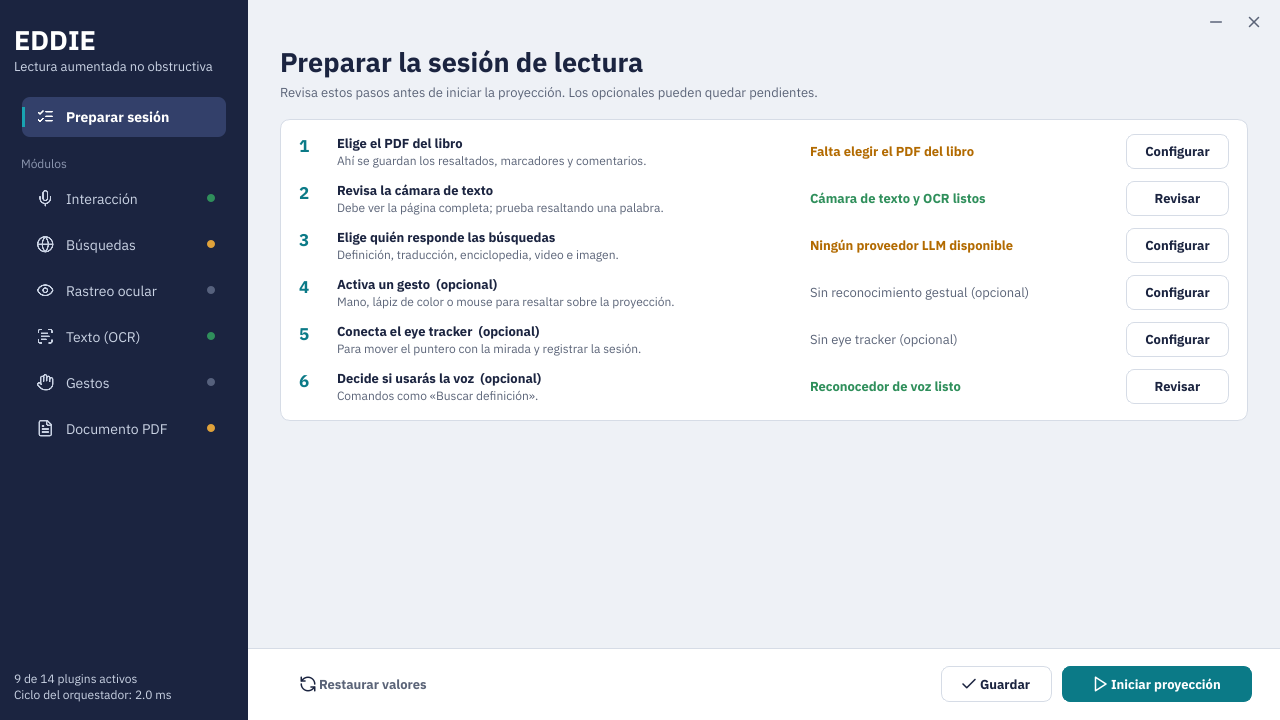
\includegraphics[width=0.85\textwidth]{figuras/00_menu_settings.png}
\caption{Pantalla de inicio con los pasos de preparación y el estado de cada módulo.}
\label{fig:ui_inicio}
\fuente{Elaboración propia (captura del avance P-07 con dispositivos simulados).}
\end{figure}

\begin{figure}[H]
\centering
\begin{minipage}{0.49\textwidth}\centering
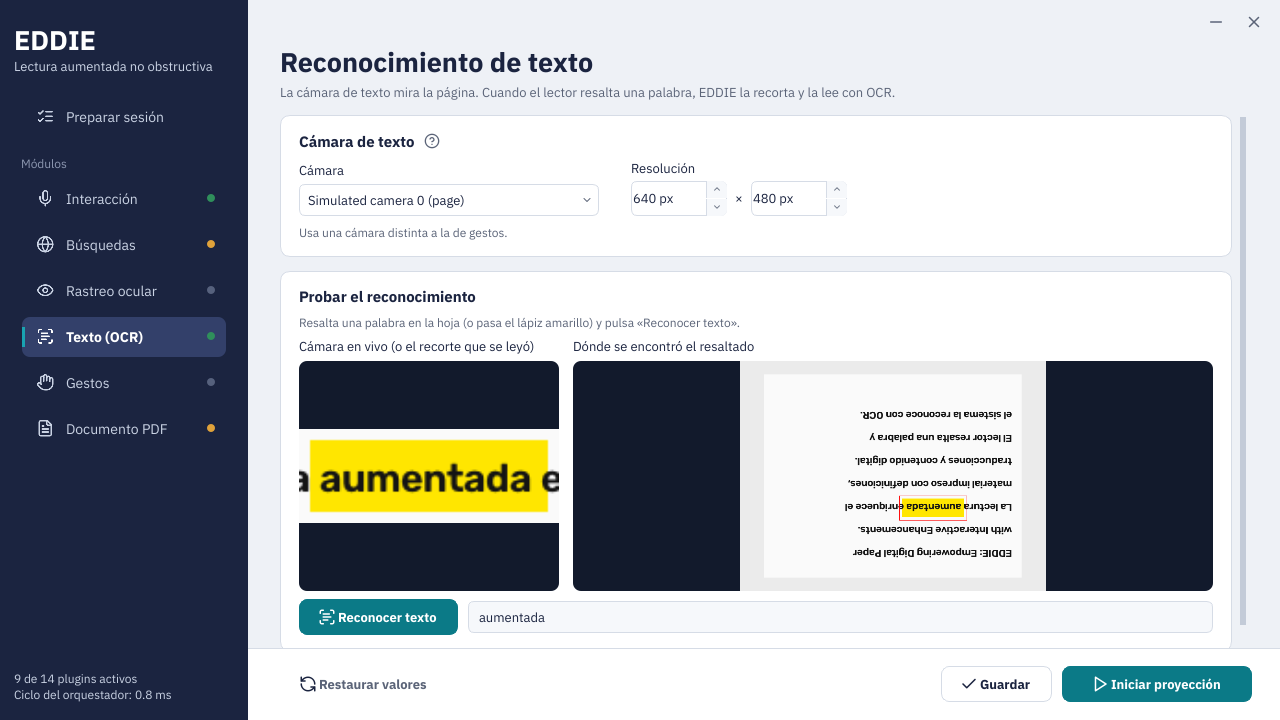
\includegraphics[width=\linewidth]{figuras/01_text.png}
\end{minipage}\hfill
\begin{minipage}{0.49\textwidth}\centering
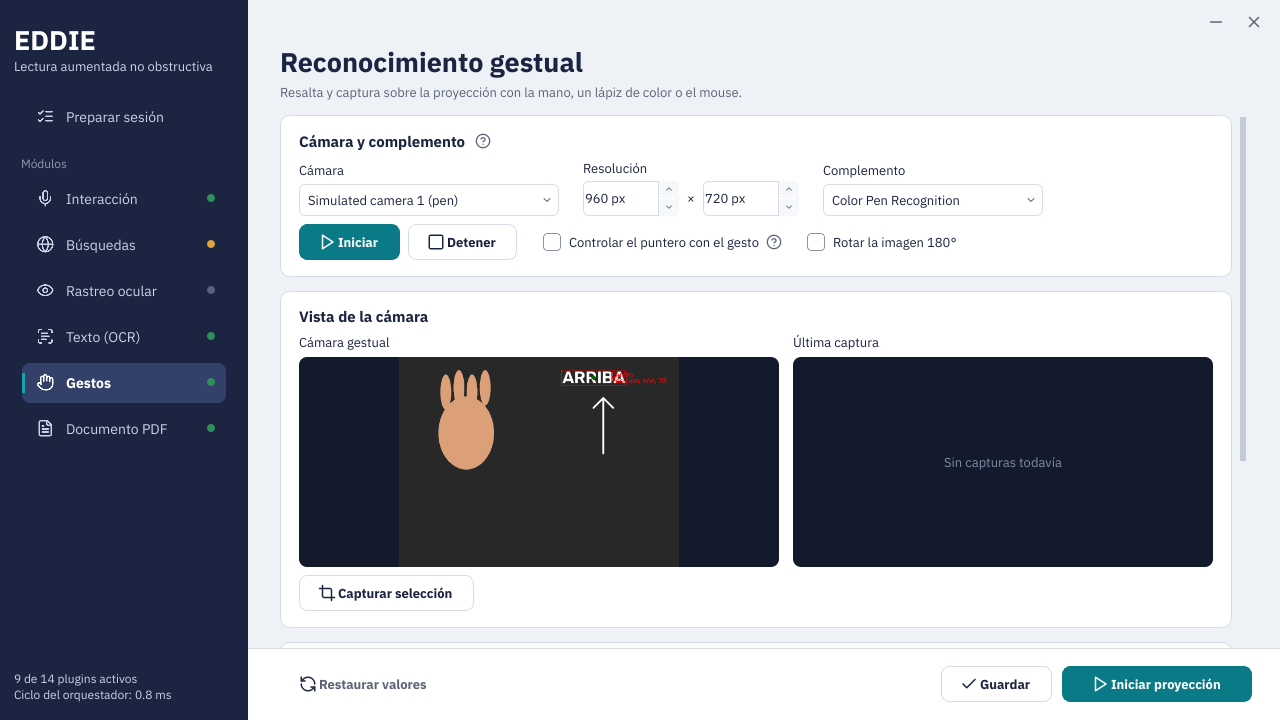
\includegraphics[width=\linewidth]{figuras/03_gesture_lapiz.png}
\end{minipage}
\caption{Configuración del reconocimiento de texto (izquierda) y de la interacción gestual con lápiz (derecha).}
\label{fig:ui_texto_gestos}
\fuente{Elaboración propia (capturas del avance P-07).}
\end{figure}

\begin{figure}[H]
\centering
\begin{minipage}{0.49\textwidth}\centering
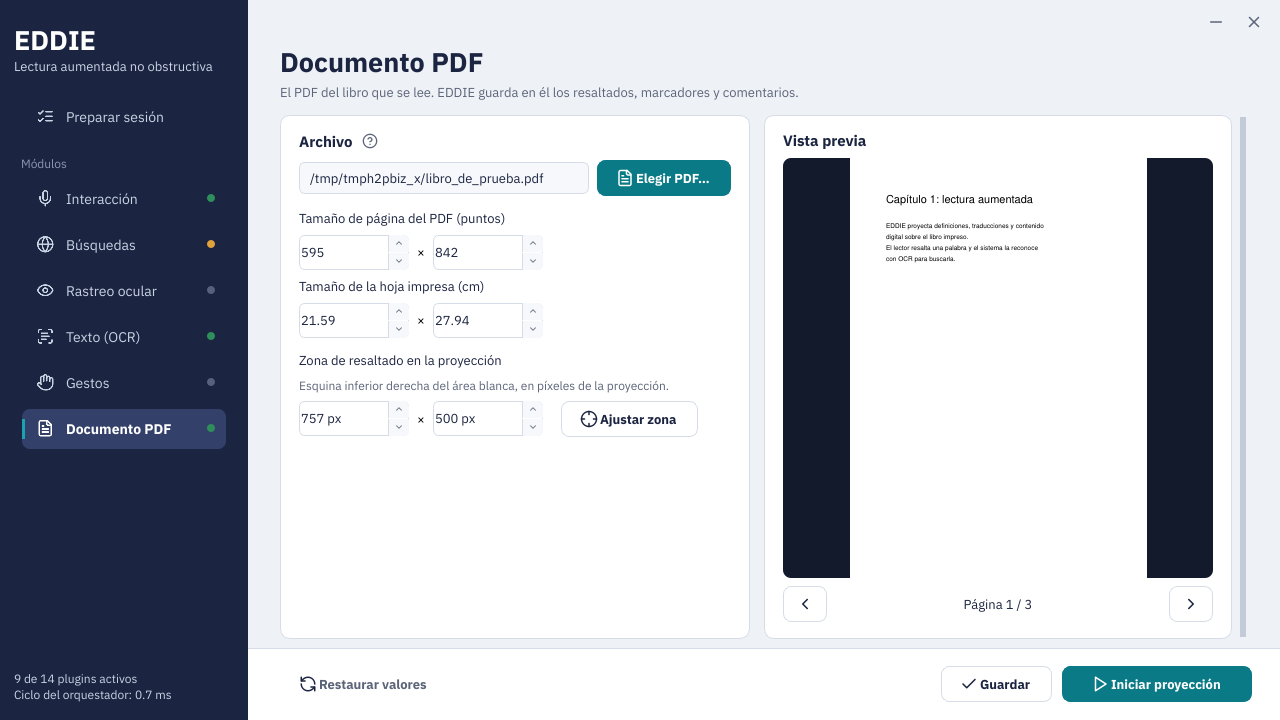
\includegraphics[width=\linewidth]{figuras/02_page.png}
\end{minipage}\hfill
\begin{minipage}{0.49\textwidth}\centering
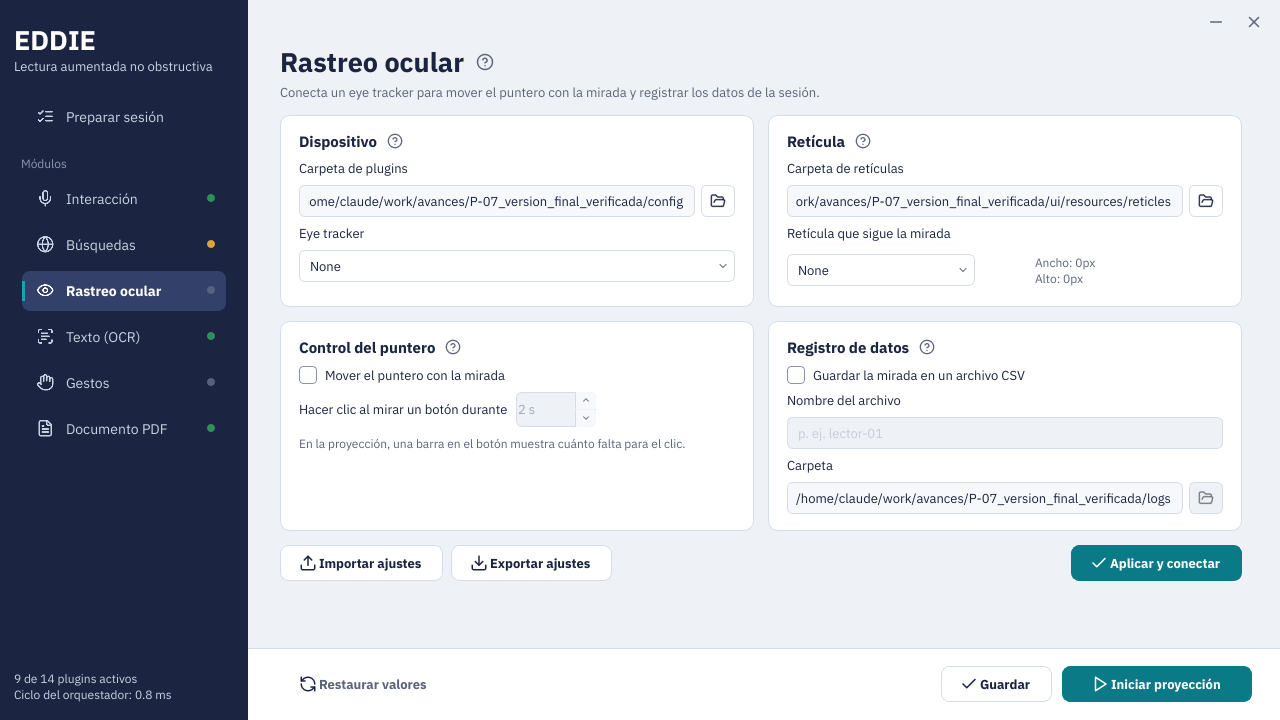
\includegraphics[width=\linewidth]{figuras/04_eye.png}
\end{minipage}
\caption{Configuración del documento PDF (izquierda) y del rastreo ocular (derecha).}
\label{fig:ui_pdf_ojo}
\fuente{Elaboración propia (capturas del avance P-07).}
\end{figure}

\begin{figure}[H]
\centering
\begin{minipage}{0.49\textwidth}\centering
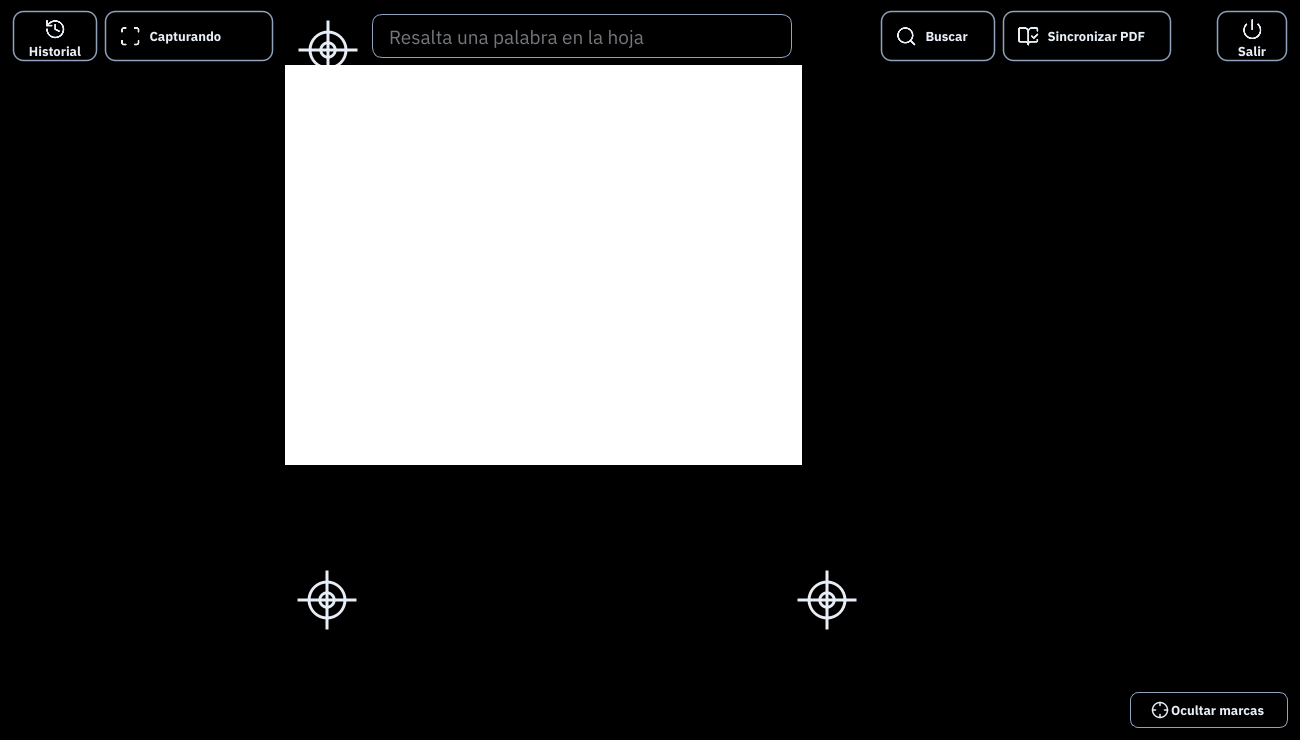
\includegraphics[width=\linewidth]{figuras/10_proyeccion.png}
\end{minipage}\hfill
\begin{minipage}{0.49\textwidth}\centering
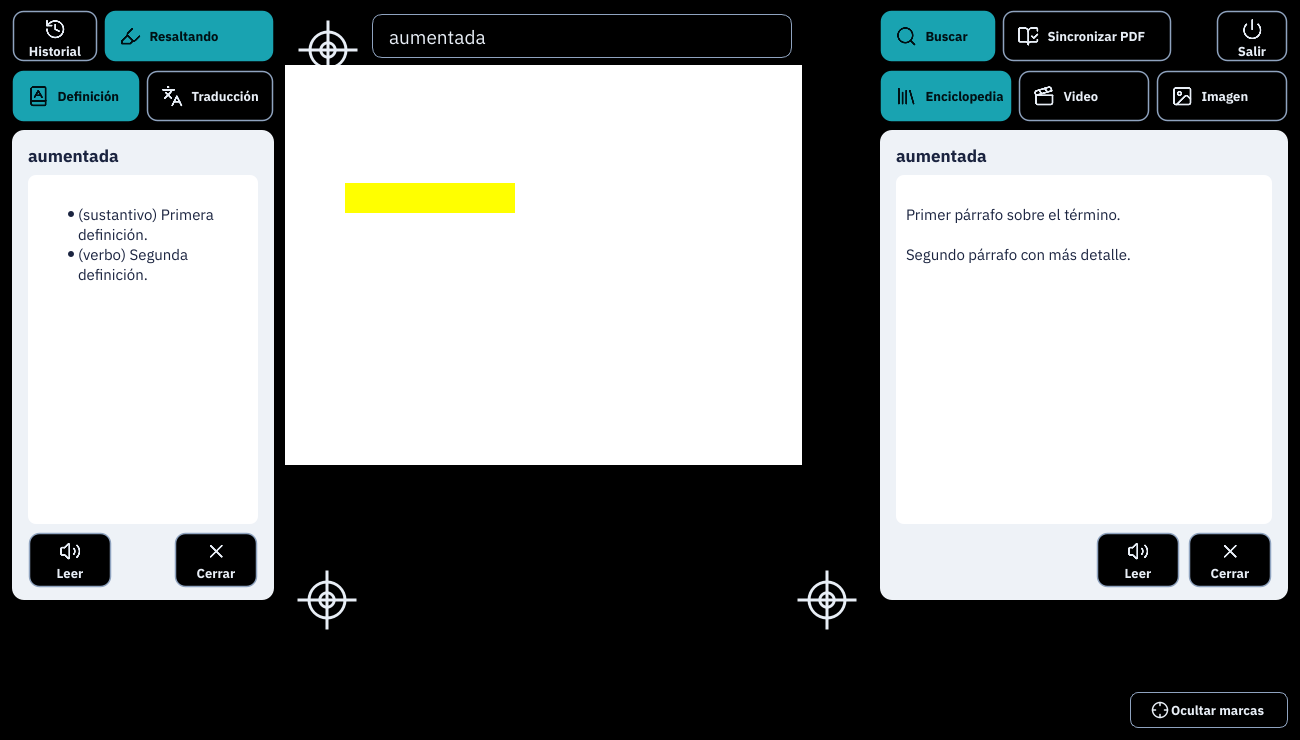
\includegraphics[width=\linewidth]{figuras/11_proyeccion_busqueda.png}
\end{minipage}
\caption{Pantalla proyectada: controles en la franja superior (izquierda) y resultado de una búsqueda (derecha).}
\label{fig:ui_proyeccion}
\fuente{Elaboración propia (capturas del avance P-07 con un modelo de lenguaje de prueba).}
\end{figure}

\section{Iteraciones de desarrollo}
\label{sec:iteraciones}

El sistema se construyó en ocho avances siguiendo RAD dentro de la etapa Do del ciclo PDCA. P-00 corresponde a los prototipos desechables del Capítulo~\ref{cap:analisis}, que confirmaron la factibilidad de cada función por separado; P-01 a P-06 son prototipos funcionales que se van sumando sobre el mismo núcleo, y P-07 es la versión verificada de las etapas Check y Act (Figura~\ref{fig:iteraciones}). A diferencia de P-00, ningún prototipo funcional se descarta: cada uno parte del código del anterior y le agrega un módulo.

El orden de integración se fijó por dependencia del hardware, de menor a mayor. Primero se construyó el núcleo, que solo usa dispositivos simulados; después la consistencia papel--PDF, que trabaja sobre archivos; luego los módulos que requieren una cámara (texto y gestos), el rastreo ocular, que depende de dispositivos y servidores externos, y al final la pantalla de proyección, que consume los resultados de todos los anteriores. Así, cuando un módulo fallaba, la causa quedaba acotada a lo recién agregado y no a lo que ya estaba probado.

\begin{figure}[H]
\centering
\begin{tikzpicture}[
  av/.style={draw=eddietinta, rounded corners=2pt, fill=eddiefondo, align=center,
             font=\scriptsize, minimum width=3.2cm, minimum height=1.25cm, inner sep=3pt},
  fin/.style={av, fill=eddieacento!15, draw=eddieacento},
  flecha/.style={-{Stealth[length=2.2mm]}, thick, eddietinta},
  fase/.style={font=\scriptsize\itshape, text=eddieacento}]
\node[av]  (p0) at (0,0)      {P-00\\ Prototipos desechables\\ semanas 1--3};
\node[av]  (p1) at (3.7,0)    {P-01\\ Núcleo y contratos\\ semanas 4--6};
\node[av]  (p2) at (7.4,0)    {P-02\\ Hardware y consistencia\\ semanas 7--8};
\node[av]  (p3) at (11.1,0)   {P-03\\ Texto e interfaz\\ semana 9};
\node[av]  (p4) at (11.1,-2.3) {P-04\\ Interacción gestual\\ semana 10};
\node[av]  (p5) at (7.4,-2.3)  {P-05\\ Rastreo ocular\\ semanas 11--12};
\node[av]  (p6) at (3.7,-2.3)  {P-06\\ Proyección, búsqueda y voz\\ semana 12};
\node[fin] (p7) at (0,-2.3)    {P-07\\ Versión verificada\\ semanas 13--17};
\draw[flecha] (p0) -- (p1);
\draw[flecha] (p1) -- (p2);
\draw[flecha] (p2) -- (p3);
\draw[flecha] (p3) -- (p4);
\draw[flecha] (p4) -- (p5);
\draw[flecha] (p5) -- (p6);
\draw[flecha] (p6) -- (p7);
\node[fase, above=1pt of p0] {Plan};
\node[fase, above=1pt of p2] {Do};
\node[fase, below=1pt of p5] {Do};
\node[fase, below=1pt of p7] {Check / Act};
\end{tikzpicture}
\caption{Secuencia de avances del desarrollo y fase del ciclo PDCA a la que pertenece cada uno.}
\label{fig:iteraciones}
\fuente{Elaboración propia a partir del plan de trabajo (Anexo~\ref{an:plan}).}
\end{figure}

Todos los avances se registran de la misma forma. Cada uno es una carpeta con su código completo y ejecutable, un archivo README\_AVANCE.md con la ficha del prototipo y la lista de lo que se revisa, y una carpeta evidencias/ que genera el script tools/generar\_evidencias.py: resultado de las pruebas, cobertura de líneas, latencia por plugin y por ciclo, estado de carga de cada plugin y capturas de la interfaz. Para pasar de un avance al siguiente se exigieron las mismas condiciones: que se cumpliera la lista de revisión del avance, que todas las pruebas automatizadas pasaran (solo se admiten fallos esperados que documentan un defecto ya conocido) y que el percentil 95 del ciclo completo siguiera bajo el umbral de 8,3~ms. Lo que un avance dejaba pendiente, y los defectos que se encontraban al usarlo, definieron el contenido del siguiente.

La Tabla~\ref{tab:avances} resume el registro de cada avance. Las subsecciones siguientes describen cada iteración con la ficha de \citet{figueroa2025arquitectura}, lo que se construyó, lo que se validó y por qué se pasó a la siguiente.

\begin{table}[H]
\centering
\caption{Registro de los avances del desarrollo.}
\label{tab:avances}
\footnotesize
\begin{tabularx}{\textwidth}{l >{\centering\arraybackslash}p{1.05cm} >{\raggedright\arraybackslash}X >{\centering\arraybackslash}p{1.05cm} >{\centering\arraybackslash}p{1.5cm} >{\centering\arraybackslash}p{1.3cm} >{\centering\arraybackslash}p{1.15cm} >{\raggedright\arraybackslash}p{1.6cm}}
\toprule
Avance & Semanas & Contenido & Pruebas & Fallos esperados & Cobertura & Ciclo p95 (ms) & Hallazgos abiertos \\ \midrule
P-00 & 1--3 & Prototipos desechables y mediciones & --- & --- & --- & --- & --- \\
P-01 & 4--6 & Núcleo orquestador y contratos & \PUnoPruebas & \PUnoXfail & \PUnoCobertura\% & \PUnoCicloPnoventaycinco & --- \\
P-02 & 7--8 & Capa de hardware y consistencia & \PDosPruebas & \PDosXfail & \PDosCobertura\% & \PDosCicloPnoventaycinco & H-02 \\
P-03 & 9 & Reconocimiento de texto e interfaz & \PTresPruebas & \PTresXfail & \PTresCobertura\% & \PTresCicloPnoventaycinco & H-02 \\
P-04 & 10 & Interacción gestual & \PCuatroPruebas & \PCuatroXfail & \PCuatroCobertura\% & \PCuatroCicloPnoventaycinco & H-01, H-02 \\
P-05 & 11--12 & Rastreo ocular & \PCincoPruebas & \PCincoXfail & \PCincoCobertura\% & \PCincoCicloPnoventaycinco & H-01, H-02 \\
P-06 & 12 & Proyección, búsqueda con LLM y voz & \PSeisPruebas & \PSeisXfail & \PSeisCobertura\% & \PSeisCicloPnoventaycinco & H-01, H-02 \\
P-07 & 13--17 & Versión final verificada & \PSietePruebas & \PSieteXfail & \PSieteCobertura\% & \PSieteCicloPnoventaycinco & Ninguno \\ \bottomrule
\end{tabularx}
\fuente{Elaboración propia a partir de evidencias/ de cada avance (dispositivos simulados). Hallazgos según la Tabla~\ref{tab:hallazgos_verif}.}
\end{table}

Los fallos esperados (\textit{xfail}) son pruebas que reproducen un defecto conocido: mientras el defecto existe la prueba se marca como fallo esperado, y en el avance que lo corrige pasa a aprobada. De este modo cada corrección queda respaldada por una prueba que demuestra el problema y su solución (Sección~\ref{sec:hallazgos}).

% ---------------------------------------------------------------------------
\subsection{P-01: Núcleo orquestador y contratos de plugins}
\label{sec:it_p01}

\paragraph{Punto de partida.} Los prototipos de P-00 mostraron que cada función de EDDIE-2023 se puede reproducir en Python, pero cada uno era un programa aislado que abría su propio dispositivo. El diagnóstico del Capítulo~\ref{cap:analisis} había identificado como causa principal de las fallas del sistema legado la coexistencia de tres mecanismos de carga distintos. Por eso la primera iteración no integra ningún módulo: construye el núcleo y los contratos a los que todos los módulos se conectarán después. La Tabla~\ref{tab:prototipo-p01} resume este avance.

% Ficha extraída de datos/tabla_prototipos.tex (P-01)
\begin{table}[H]
\centering
\caption{Primer prototipo - Núcleo orquestador y contratos de plugins.}
\label{tab:prototipo-p01}
\small
\begin{tabularx}{\textwidth}{>{\bfseries}l X}
\toprule
ID Prototipo & P-01 \\ \midrule
Nombre & Núcleo orquestador y contratos de plugins \\ \midrule
Objetivos & Definir PluginBase y los contratos de cada módulo (ICameraSensor, IImageProcessor, IGesturePlugin, IEyeTracker, IConsistencyProvider, IWebSearchProvider, ISpeechProvider). \newline Implementar el OrchestratorCore (inicializar $\rightarrow$ ejecutar $\rightarrow$ liberar) y el PluginLoader con un único mecanismo de carga. \newline Validar la inyección de dependencias sensor$\rightarrow$consumidor, el aislamiento de fallos y la latencia por ciclo. \\ \midrule
Descripción & Primera versión del núcleo, sin interfaz. Se prueba con dispositivos simulados (MockCameraSensor, EyeTrackerMock) y con plugins de prueba: un consumidor de frames, un consumidor de resultados del ciclo, un plugin que falla cada 10 ciclos y una entrada con una clase inexistente (equivalente a la DLL faltante de los errores E38/E50). El OrchestratorCore de este avance es la versión temprana del repositorio (sin overrides, invoke ni reinicio en caliente). \\ \midrule
Requisitos Funcionales & N1, N2, N3, RFCO12 \\ \midrule
Requisitos No Funcionales & RNF-01, RNF-02, RNF-04, RNF-05 \\ \bottomrule
\end{tabularx}
\fuente{Elaboración propia, 2026.}
\end{table}


\paragraph{Desarrollo.} Se definió PluginBase y un contrato por tipo de módulo (Tabla~\ref{tab:contratos}), el PluginLoader con un único mecanismo de carga basado en importlib y la primera versión del OrchestratorCore con su ciclo inicializar--ejecutar--liberar. Como todavía no existían módulos reales, el núcleo se probó con dispositivos simulados (MockCameraSensor y EyeTrackerMock) y con plugins de prueba construidos para forzar los casos difíciles: un consumidor de frames, un consumidor de los resultados del ciclo, un plugin que falla a propósito cada 10 ciclos y una entrada de configuración que apunta a una clase inexistente, equivalente a la DLL faltante de los errores E38 y E50 de \citet{ibaceta2023evaluacion}.

\paragraph{Registro y validación.} En una ejecución de 300 ciclos, los cinco plugins válidos quedaron inicializados y la clase inexistente quedó registrada como load\_failed sin detener el arranque. La falla inyectada en los ciclos 10, 20, 30, \ldots{} quedó aislada: los demás plugins entregaron resultado en todos los ciclos. Se aprobaron \PUnoPruebas{} pruebas, con una cobertura de \PUnoCobertura\% y un ciclo completo de \PUnoCicloPnoventaycinco~ms en el percentil 95, lejos del umbral de 8,3~ms.

\paragraph{Paso a la siguiente iteración.} El núcleo cumplía su función, pero solo con dispositivos simulados y sin formas de operar un plugin fuera del ciclo. Para integrar el primer módulo real faltaban dos cosas: una capa que permitiera cambiar cada dispositivo entre real y simulado sin modificar código, y operaciones para invocar, reiniciar y detener plugins bajo demanda, que la consistencia y la interfaz necesitarían. Ambas definieron P-02.

% ---------------------------------------------------------------------------
\subsection{P-02: Capa de abstracción de hardware y módulo de consistencia}
\label{sec:it_p02}

\paragraph{Punto de partida.} Con el núcleo validado, se eligió como primer módulo la consistencia papel--PDF porque es el único que no depende de una cámara para probarse: sus entradas pueden ser imágenes de la hoja y su salida es un archivo PDF. Esto permitía validar la integración de un módulo completo sin introducir todavía las variables del hardware (Tabla~\ref{tab:prototipo-p02}).

% Ficha extraída de datos/tabla_prototipos.tex (P-02)
\begin{table}[H]
\centering
\caption{Segundo prototipo - Capa de abstracción de hardware y módulo de consistencia.}
\label{tab:prototipo-p02}
\small
\begin{tabularx}{\textwidth}{>{\bfseries}l X}
\toprule
ID Prototipo & P-02 \\ \midrule
Nombre & Capa de abstracción de hardware y módulo de consistencia \\ \midrule
Objetivos & Incorporar DeviceFactory para conmutar cada dispositivo entre real y simulado sin cambiar código. \newline Implementar la cámara real (OpenCV, hilo de captura) y la enumeración de cámaras de Windows. \newline Integrar primero el módulo sin dependencia de hardware: la consistencia papel$\leftrightarrow$PDF como plugin IConsistencyProvider (PyMuPDF). \newline Extender el núcleo con overrides de configuración, invocación bajo demanda, reinicio en caliente y traza de ejecución. \\ \midrule
Descripción & El núcleo pasa a su versión definitiva y se agrega la capa HAL. La consistencia (resaltados, marcadores, comentarios y figuras, búsqueda de texto) se ejecuta a través del orquestador con OrchestratorCore.invoke(). Sigue sin interfaz: se demuestra con demos/demo\_consistencia.py, que sincroniza tres <<fotos>> sintéticas de la hoja con un PDF de prueba y guarda el PDF resultante y el render de cada página. \\ \midrule
Requisitos Funcionales & N4, N5, N6, N8, C1, C2, C3, C7, C9, C10, C11 (parcial) \\ \midrule
Requisitos No Funcionales & RNF-01, RNF-02, RNF-04, RNF-05 \\ \bottomrule
\end{tabularx}
\fuente{Elaboración propia, 2026.}
\end{table}


\paragraph{Desarrollo.} Se incorporó DeviceFactory, que entrega la implementación real o simulada de cada dispositivo según la variable EDDIE\_DEVICE\_MODE, junto con la cámara real (OpenCV con un hilo de captura) y la enumeración de cámaras de Windows. El núcleo pasó a su versión definitiva con las operaciones invoke, restart\_plugin y stop\_plugin, la sobrescritura de la configuración y la traza de ejecución. La consistencia se integró como plugin IConsistencyProvider sobre PyMuPDF. Como el avance todavía no tenía interfaz, se demostró con un script que sincroniza tres fotografías sintéticas de la hoja con un PDF de prueba: un marcador azul, una nota adhesiva y figuras magenta (Figura~\ref{fig:p02_frames}).

\begin{figure}[H]
\centering
\begin{minipage}[t]{0.31\textwidth}\centering

\includegraphics[width=\linewidth]{figuras/frame_marcador.png}\\[-2pt]{\footnotesize (a) Marcador}
\end{minipage}\hfill
\begin{minipage}[t]{0.31\textwidth}\centering

\includegraphics[width=\linewidth]{figuras/frame_comentario.png}\\[-2pt]{\footnotesize (b) Nota adhesiva}
\end{minipage}\hfill
\begin{minipage}[t]{0.31\textwidth}\centering
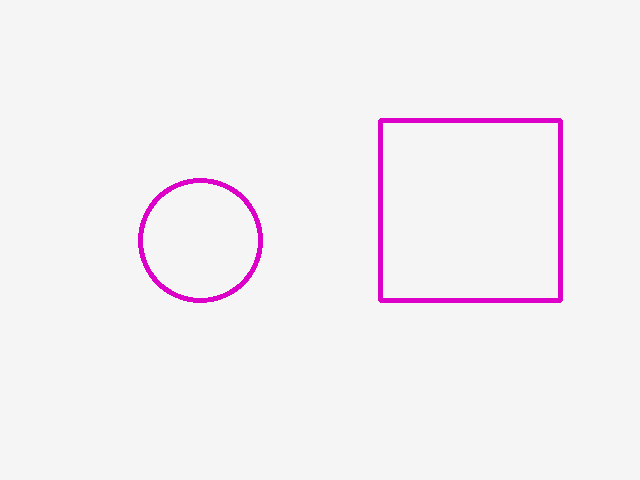
\includegraphics[width=\linewidth]{figuras/frame_figuras.png}\\[-2pt]{\footnotesize (c) Figuras}
\end{minipage}
\caption{Imágenes de la hoja usadas en la demostración de consistencia de P-02.}
\label{fig:p02_frames}
\fuente{Elaboración propia (evidencias/consistencia de P-02).}
\end{figure}

\paragraph{Registro y validación.} Las diez llamadas de la demostración se ejecutaron correctamente a través del orquestador y el documento en memoria quedó con el marcador, el comentario y las figuras. Sin embargo, la lista de revisión incluía reabrir el PDF guardado, y ahí apareció el primer hallazgo: el archivo en disco había perdido parte de los cambios (Tabla~\ref{tab:persistencia}). La causa era el guardado incremental de PyMuPDF, que desde el segundo guardado dejaba dañada la tabla de referencias del PDF (H-02). El defecto se registró con una prueba marcada como fallo esperado y se dejó para la verificación, porque no impedía seguir integrando módulos. El avance cerró con \PDosPruebas{} pruebas aprobadas, \PDosXfail{} fallo esperado y una cobertura de \PDosCobertura\%, que baja respecto de P-01 porque el código de los dispositivos reales todavía no tenía pruebas que lo recorrieran.

\begin{table}[H]
\centering
\caption{Persistencia de la demostración de consistencia al reabrir el PDF guardado.}
\label{tab:persistencia}
\small
\begin{tabular}{l c c c}
\toprule
Avance & Anotaciones por página & Marcadores & PDF reparado al abrir \\ \midrule
Esperado & 1, 1, 2 & 2 & No \\
P-02 & 0, 0, 2 & 0 & Sí \\
P-07 & 1, 1, 2 & 2 & No \\ \bottomrule
\end{tabular}
\fuente{Elaboración propia (evidencias/consistencia/reporte.json de P-02 y P-07).}
\end{table}

\paragraph{Paso a la siguiente iteración.} La consistencia funcionaba, pero solo podía operarse desde un script. Para que un investigador la usara hacía falta la interfaz, y el siguiente módulo en orden de dependencia era el reconocimiento de texto, que necesita una sola cámara. Ambos se abordaron juntos en P-03, porque la interfaz permitía además probar el OCR sin esperar la pantalla de proyección.

% ---------------------------------------------------------------------------
\subsection{P-03: Reconocimiento de texto e interfaz de configuración}
\label{sec:it_p03}

\paragraph{Punto de partida.} En esta iteración aparece la interfaz y se integra el primer módulo que depende de una cámara: el reconocimiento del texto resaltado (Tabla~\ref{tab:prototipo-p03}).

% Ficha extraída de datos/tabla_prototipos.tex (P-03)
\begin{table}[H]
\centering
\caption{Tercer prototipo - Reconocimiento de texto e interfaz de configuración.}
\label{tab:prototipo-p03}
\small
\begin{tabularx}{\textwidth}{>{\bfseries}l X}
\toprule
ID Prototipo & P-03 \\ \midrule
Nombre & Reconocimiento de texto e interfaz de configuración \\ \midrule
Objetivos & Integrar el reconocimiento del texto resaltado (IImageProcessor: segmentación del resaltado + Tesseract) sobre la cámara de texto declarada. \newline Construir la ventana de configuración a partir de los controles extraídos de los .Designer.cs, con un diseño propio en español (ui/theme.py, ui/modern\_forms.py) y las páginas Texto (OCR) y Documento PDF. \newline Ejecutar el ciclo del orquestador dentro de Qt (EddieRuntime) y persistir los ajustes. \newline Poder probar el OCR y ver el PDF cargado desde estas páginas, sin esperar la pantalla de proyección. \\ \midrule
Descripción & Aparece la interfaz. Conserva todos los controles del original (mismo nombre, tipo, rangos y estado inicial), ordenados en tarjetas con layouts de Qt, con un menú lateral que muestra el estado de cada módulo y una pantalla de inicio <<Preparar sesión>>. Solo se construyen las páginas de los módulos ya integrados: las demás aparecen en el menú deshabilitadas con el avance en que se integran, y <<Iniciar proyección>> avisa que la proyección llega en P-06. Como en el C\# el texto reconocido solo se veía desde la proyección, se agregan el botón <<Reconocer texto>> con el texto reconocido y una vista previa del PDF con navegación de páginas. Los mensajes son avisos no modales. \\ \midrule
Requisitos Funcionales & FD1, N7, U1, U3, RFS3, RFS5, RFS6, RFS7, RFS8 \\ \midrule
Requisitos No Funcionales & RNF-01, RNF-06, RNF-07 \\ \bottomrule
\end{tabularx}
\fuente{Elaboración propia, 2026.}
\end{table}


\paragraph{Desarrollo.} El reconocimiento de texto se integró como plugin IImageProcessor sobre la cámara de texto declarada, con la segmentación del resaltado y Tesseract validados en P-00. La ventana de configuración se construyó a partir de los controles extraídos de los archivos .Designer.cs de EDDIE-2023, con su mismo nombre, tipo, rango y estado inicial, ordenados en tarjetas y en español (Figura~\ref{fig:ui_inicio}). El ciclo del orquestador pasó a ejecutarse dentro de Qt y los ajustes se guardan en config/user\_settings.json. Como en el sistema original el texto reconocido solo se veía en la proyección, se agregaron el botón «Reconocer texto» y una vista previa del PDF, de modo que ambos módulos pudieran probarse en este mismo avance.

Una decisión de esta iteración fue mostrar, en cada avance, solo los módulos ya integrados. Los demás aparecen deshabilitados con el avance en que se integran, tanto en el menú lateral como en la pantalla «Preparar sesión» (Figura~\ref{fig:p03_inicio}). Así la interfaz nunca ofrece una función que todavía no existe y el estado del desarrollo queda visible en la propia aplicación.

\begin{figure}[H]
\centering
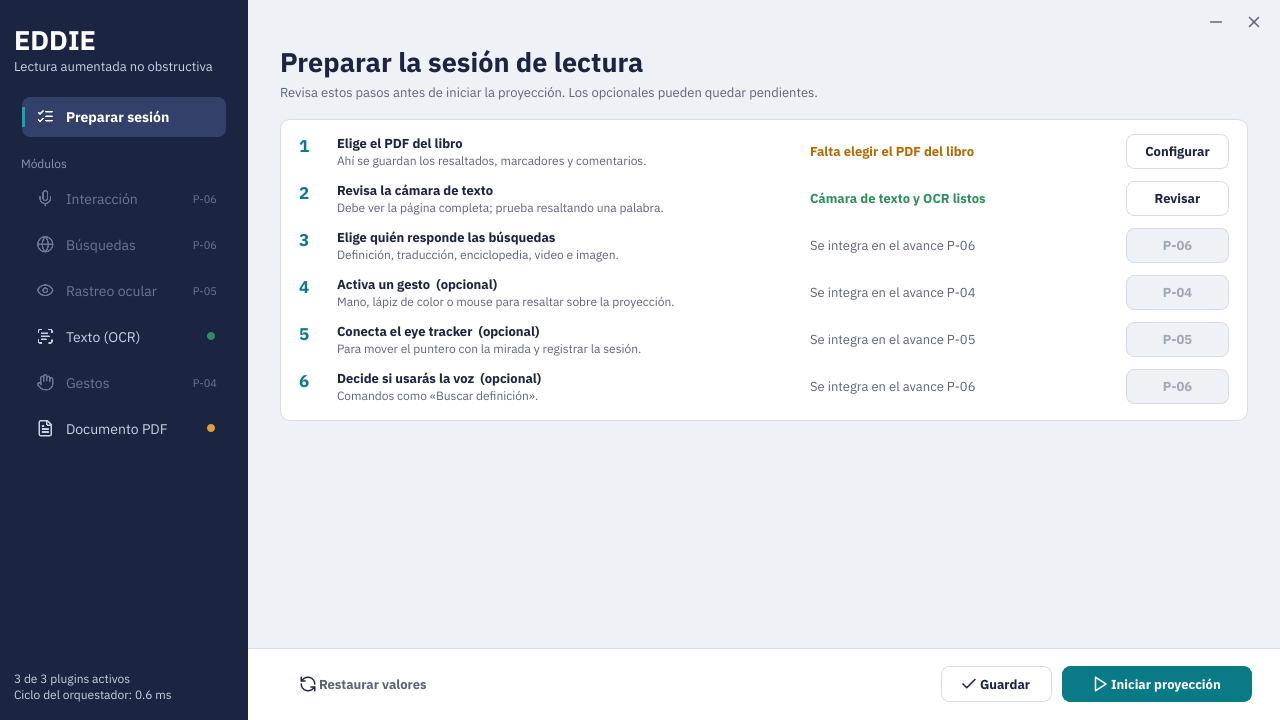
\includegraphics[width=0.85\textwidth]{figuras/p03_inicio.png}
\caption{Pantalla «Preparar sesión» en P-03: los módulos pendientes aparecen deshabilitados con el avance en que se integran.}
\label{fig:p03_inicio}
\fuente{Elaboración propia (evidencias/capturas de P-03).}
\end{figure}

\paragraph{Registro y validación.} Se verificó que «Reconocer texto» marcara el resaltado y mostrara el texto leído, que la vista del PDF permitiera recorrerlo y rechazara un archivo dañado con un aviso sin cerrarse, que cada control existiera con las propiedades del original y que Guardar y Restaurar valores persistieran los ajustes. El avance cerró con \PTresPruebas{} pruebas aprobadas. La cobertura bajó a \PTresCobertura\% porque el código de la interfaz todavía no tenía pruebas de flujo completas; H-02 seguía abierto.

\paragraph{Paso a la siguiente iteración.} Con texto e interfaz operativos, el sistema ya permitía leer un documento, pero no interactuar con él sobre el papel. La interacción gestual era el paso siguiente: usa una segunda cámara, agrega la calibración entre el sensor y la aplicación, y produce la captura de selección que más tarde necesitaría la búsqueda por imagen.

% ---------------------------------------------------------------------------
\subsection{P-04: Interacción gestual}
\label{sec:it_p04}

\paragraph{Punto de partida.} Esta iteración integra los tres detectores gestuales de EDDIE-2023 (lápiz de color, mano y mouse) bajo el contrato IGesturePlugin, compartiendo la cámara gestual (Tabla~\ref{tab:prototipo-p04}).

% Ficha extraída de datos/tabla_prototipos.tex (P-04)
\begin{table}[H]
\centering
\caption{Cuarto prototipo - Interacción gestual.}
\label{tab:prototipo-p04}
\small
\begin{tabularx}{\textwidth}{>{\bfseries}l X}
\toprule
ID Prototipo & P-04 \\ \midrule
Nombre & Interacción gestual \\ \midrule
Objetivos & Integrar los plugins gestuales del C\# (Color Pen, Hand Skin, Mouse) bajo IGesturePlugin, compartiendo la cámara gestual declarada. \newline Portar la calibración sensor$\rightarrow$aplicación, el control del cursor (<<Recognition on>>), la máquina de estados del clic y la captura automática de la selección. \newline Agregar la página Gestos, con calibración asistida (<<Fijar inicio>> / <<Fijar fin>> desde la lectura del sensor). \\ \midrule
Descripción & Los tres detectores heredan una base común (CalibratedGesturePlugin) que aplica la calibración y el clic; cada uno solo implementa su detección. Este avance porta el comportamiento del C\# tal cual, incluida la rotación fija de 180$^{\circ}$ de Hand Skin, que después se detectó como defecto (H-01). \\ \midrule
Requisitos Funcionales & G1, G2, G3, U2 \\ \midrule
Requisitos No Funcionales & RNF-01, RNF-04, RNF-06 \\ \bottomrule
\end{tabularx}
\fuente{Elaboración propia, 2026.}
\end{table}


\paragraph{Desarrollo.} Los tres detectores heredan una base común, CalibratedGesturePlugin, que aplica la calibración y la máquina de estados del clic; cada uno implementa solo su detección. Se agregó la página Gestos con calibración asistida: los botones «Fijar inicio» y «Fijar fin» copian la lectura actual del sensor, una función nueva respecto del original. Este avance portó el comportamiento del C\# tal como estaba, incluida la rotación fija de 180° del detector de mano.

\paragraph{Registro y validación.} Las pruebas confirmaron que el lápiz simulado mueve las coordenadas, que la calibración las transforma al espacio de la aplicación, que al soltar el lápiz se captura la selección y que los tres plugins se reconectan al reiniciar la cámara. El ciclo completo subió a \PCuatroCicloPnoventaycinco~ms en el percentil 95 por el procesamiento de imagen de ColorPenRecognition, todavía bajo el umbral. Al calibrar con la mano apareció el segundo hallazgo: la vista de la cámara se mostraba invertida (Figura~\ref{fig:p04_mano}). HandSkinRecognition.cs rotaba siempre la imagen porque la cámara del laboratorio estaba montada al revés, y el port había conservado esa rotación fija (H-01). Se registró como fallo esperado y quedó para la verificación. El avance cerró con \PCuatroPruebas{} pruebas aprobadas y \PCuatroXfail{} fallo esperado.

\begin{figure}[H]
\centering
\begin{minipage}[t]{0.49\textwidth}\centering
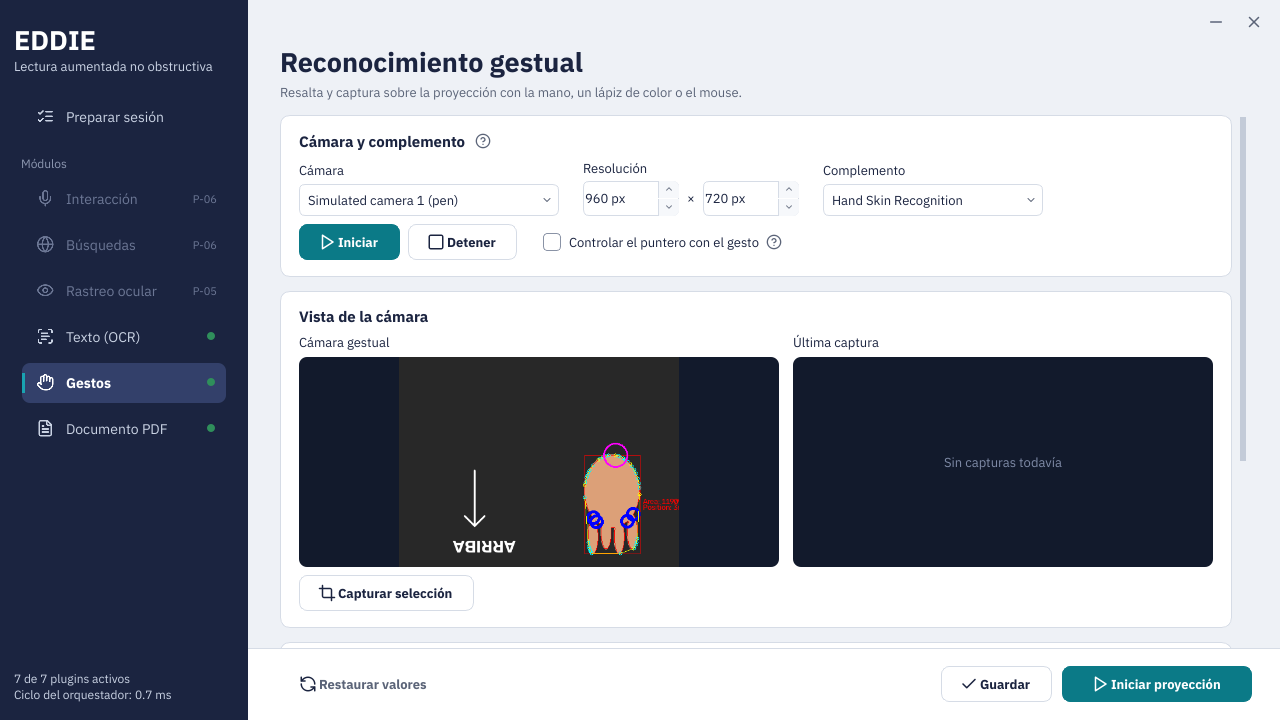
\includegraphics[width=\linewidth]{figuras/p04_gesto_mano.png}\\[-2pt]{\footnotesize (a) P-04: imagen rotada 180°}
\end{minipage}\hfill
\begin{minipage}[t]{0.49\textwidth}\centering
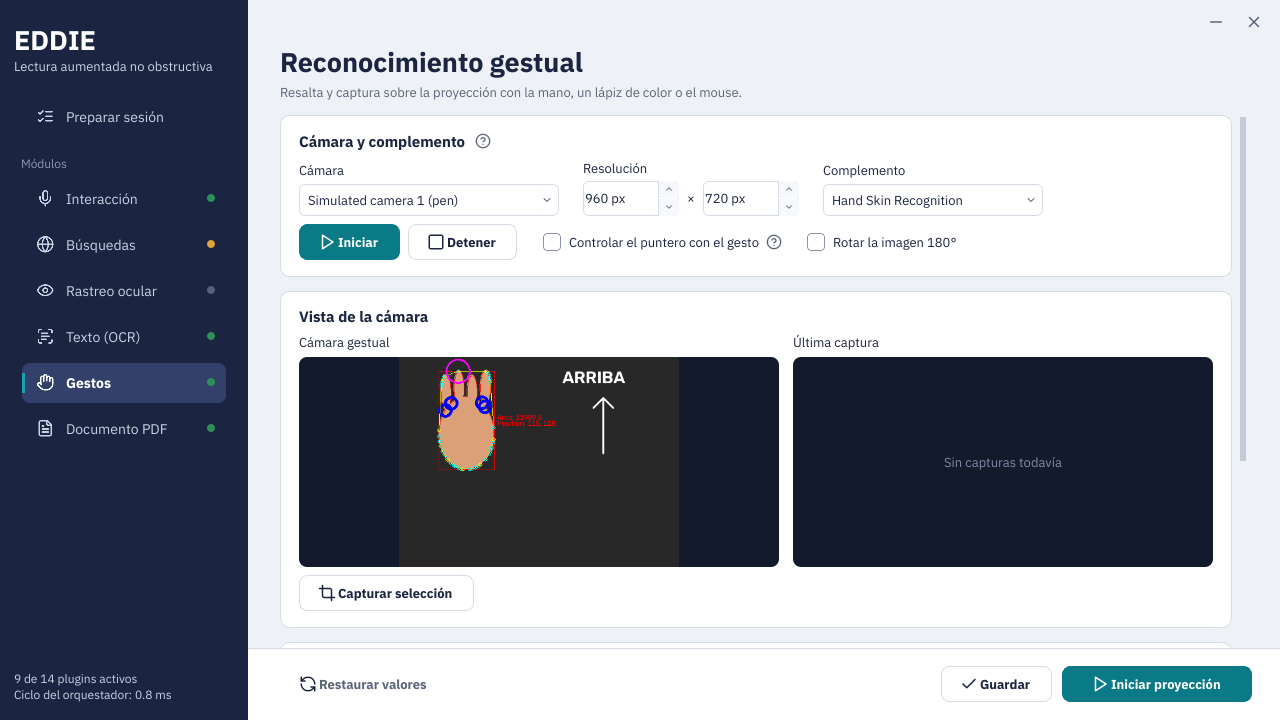
\includegraphics[width=\linewidth]{figuras/03_gesture_mano.png}\\[-2pt]{\footnotesize (b) P-07: orientación corregida}
\end{minipage}
\caption{Página Gestos con el detector de mano antes y después de corregir H-01. La escena simulada incluye el rótulo «ARRIBA» para detectar la inversión.}
\label{fig:p04_mano}
\fuente{Elaboración propia (evidencias/capturas de P-04 y P-07).}
\end{figure}

\paragraph{Paso a la siguiente iteración.} Con texto y gestos integrados quedaba el módulo con mayor dependencia del hardware: el rastreo ocular, que se conecta con dispositivos y servidores externos. Se dejó para después de las cámaras porque, si los eye trackers no se lograban integrar a tiempo, el plan de trabajo preveía validarlo con el dispositivo simulado sin bloquear los demás módulos.

% ---------------------------------------------------------------------------
\subsection{P-05: Rastreo ocular}
\label{sec:it_p05}

\paragraph{Punto de partida.} Esta iteración unifica bajo IEyeTracker los tres dispositivos que usaba EDDIE-2023 (GazePoint, TheEyeTribe y GazeCloud), con EyeTrackerMock como contingencia (Tabla~\ref{tab:prototipo-p05}).

% Ficha extraída de datos/tabla_prototipos.tex (P-05)
\begin{table}[H]
\centering
\caption{Quinto prototipo - Rastreo ocular.}
\label{tab:prototipo-p05}
\small
\begin{tabularx}{\textwidth}{>{\bfseries}l X}
\toprule
ID Prototipo & P-05 \\ \midrule
Nombre & Rastreo ocular \\ \midrule
Objetivos & Unificar GazePoint (Open Gaze API), TheEyeTribe y GazeCloud bajo IEyeTracker, con EyeTrackerMock como contingencia (DeviceFactory). \newline Portar la sesión de mirada: control del mouse por mirada, clic por permanencia, retícula y registro CSV. \newline Agregar la página Rastreo ocular (exportar/importar configuración). \\ \midrule
Descripción & Los tres protocolos se prueban con servidores falsos que emiten el mismo formato que los dispositivos reales. La sesión de mirada es un consumidor de resultados del ciclo: recibe la muestra del eye tracker en el mismo ciclo en que se produce. \\ \midrule
Requisitos Funcionales & RO1–RO7, RFS4 \\ \midrule
Requisitos No Funcionales & RNF-01, RNF-02, RNF-05 \\ \bottomrule
\end{tabularx}
\fuente{Elaboración propia, 2026.}
\end{table}


\paragraph{Desarrollo.} Cada protocolo se implementó como un plugin que entrega muestras de mirada normalizadas. Para probarlos sin el hardware se construyeron servidores falsos que emiten el mismo formato que los dispositivos reales. La sesión de mirada (control del puntero, clic por permanencia, retícula y registro CSV) se implementó como consumidor de los resultados del ciclo, por lo que recibe cada muestra en el mismo ciclo en que se produce. Se agregó la página Rastreo ocular, con exportación e importación de la configuración usando las mismas claves del C\# (Figura~\ref{fig:ui_pdf_ojo}).

\paragraph{Registro y validación.} Se comprobó que cada protocolo entrega muestras normalizadas, que un eye tracker sin dispositivo falla la inicialización sin afectar al resto y que «Aplicar y conectar» con el dispositivo simulado muestra la retícula y escribe el CSV de la sesión. Al ejecutar el avance en el computador de desarrollo apareció un tercer hallazgo: cada clic en los botones de carpeta y las casillas de esta página dejaba una excepción en el registro, aunque la acción se ejecutaba (H-03). A diferencia de los anteriores, se corrigió en el mismo avance, que es el primero que tiene esos controles, y se agregó una prueba que lo detecta. El avance cerró con \PCincoPruebas{} pruebas aprobadas y \PCincoXfail{} fallo esperado, correspondiente a H-01.

\paragraph{Paso a la siguiente iteración.} Con todas las entradas integradas (texto, gestos y mirada), faltaba la pantalla de proyección que las combina frente al lector, junto con la búsqueda y la voz, que dependen de sus resultados: el término reconocido, la imagen capturada con el gesto y la selección por mirada.

% ---------------------------------------------------------------------------
\subsection{P-06: Pantalla de proyección, búsqueda con LLM y voz}
\label{sec:it_p06}

\paragraph{Punto de partida.} Esta iteración completa el sistema: integra la pantalla de proyección, los servicios de búsqueda y la voz (Tabla~\ref{tab:prototipo-p06}).

% Ficha extraída de datos/tabla_prototipos.tex (P-06)
\begin{table}[H]
\centering
\caption{Sexto prototipo - Pantalla de proyección, búsqueda con LLM y voz.}
\label{tab:prototipo-p06}
\small
\begin{tabularx}{\textwidth}{>{\bfseries}l X}
\toprule
ID Prototipo & P-06 \\ \midrule
Nombre & Pantalla de proyección, búsqueda con LLM y voz \\ \midrule
Objetivos & Integrar la pantalla de proyección (ProjectionScreenActivity2): modo resaltado/captura, búsqueda y sincronización papel$\leftrightarrow$PDF, con los botones en la franja superior (zona de mayor validez del eye tracker según Ibaceta, 2023) y la zona de lectura y las cruces en su posición original. \newline Responder los cinco servicios de búsqueda con Gemini 2.5 Flash bajo IWebSearchProvider, en lugar de las APIs vencidas (Wikipedia, Google, Bing, YouTube, Cloud Vision). \newline Integrar lectura en voz alta y comandos de voz (ISpeechProvider) y las páginas Interacción y Búsquedas. \\ \midrule
Descripción & Con este avance el sistema queda completo y equivale al código de <<Proyecto final>> antes de la verificación. Es una extensión respecto del alcance del seminario, donde IWebSearchProvider quedaba solo como interfaz. \\ \midrule
Requisitos Funcionales & B1–B13, C5, C6, C8, C11, C12, RFS1, RFS2 \\ \midrule
Requisitos No Funcionales & RNF-01, RNF-06, RNF-08 \\ \bottomrule
\end{tabularx}
\fuente{Elaboración propia, 2026.}
\end{table}


\paragraph{Desarrollo.} La pantalla de proyección reúne el modo de resaltado y captura, la búsqueda y la sincronización papel--PDF. Sus botones se ubicaron en la franja superior, la zona de mayor validez del eye tracker según \citet{ibaceta2023evaluacion}, y la zona de lectura y las cruces de calibración conservan su posición original (Figura~\ref{fig:ui_proyeccion}). Los cinco servicios de búsqueda de EDDIE-2023 dependían de APIs que ya no funcionan; en esta iteración se responden con un modelo de lenguaje (Gemini 2.5 Flash) bajo el contrato IWebSearchProvider. Se integraron además la lectura en voz alta y los comandos de voz bajo ISpeechProvider, y las páginas Interacción y Búsquedas. La Figura~\ref{fig:p06_proyeccion} muestra dos funciones que aparecen por primera vez en este avance: el sincronizador del PDF y el historial de búsquedas.

\begin{figure}[H]
\centering
\begin{minipage}[t]{0.49\textwidth}\centering
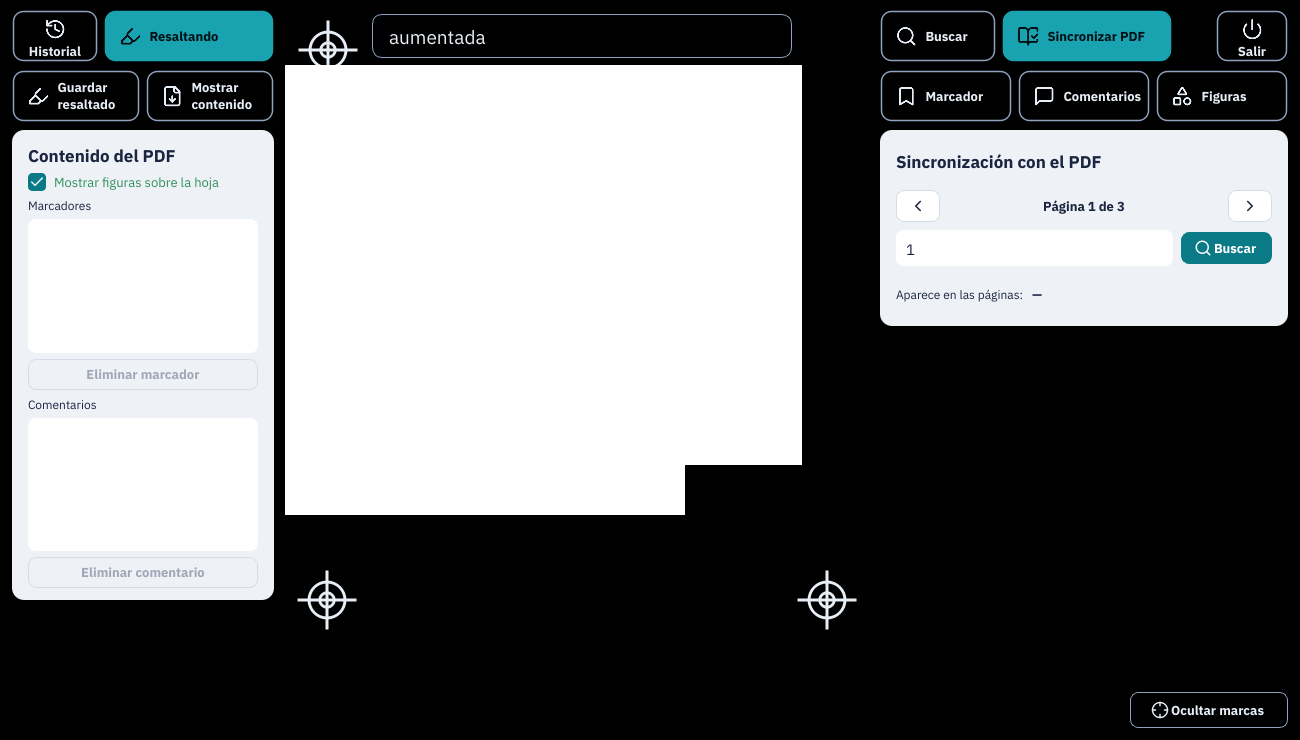
\includegraphics[width=\linewidth]{figuras/12_proyeccion_pdf.png}\\[-2pt]{\footnotesize (a) Sincronizador del PDF}
\end{minipage}\hfill
\begin{minipage}[t]{0.49\textwidth}\centering
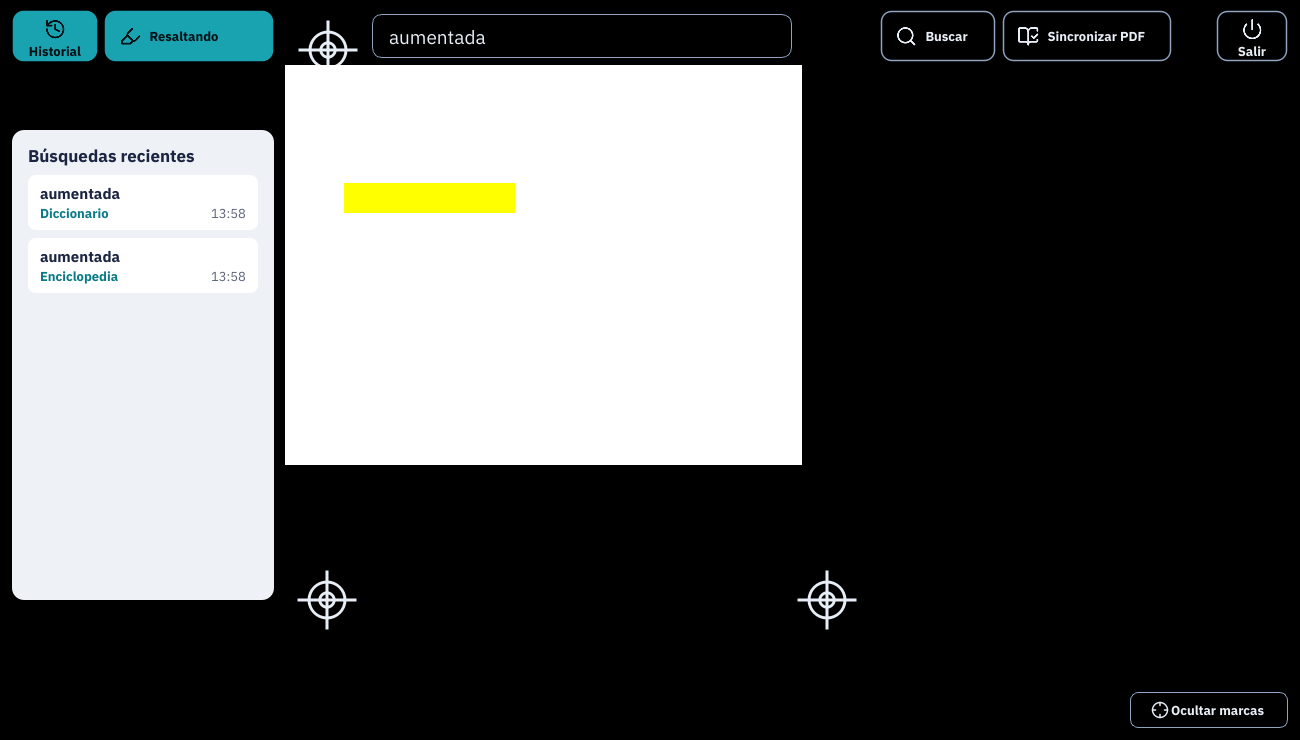
\includegraphics[width=\linewidth]{figuras/13_proyeccion_historial.png}\\[-2pt]{\footnotesize (b) Historial de búsquedas}
\end{minipage}
\caption{Pantalla de proyección de P-06.}
\label{fig:p06_proyeccion}
\fuente{Elaboración propia (evidencias/capturas de P-06, con un modelo de lenguaje de prueba).}
\end{figure}

\paragraph{Registro y validación.} Se probó el flujo completo: resaltar, reconocer el texto, corregir el término, pedir la definición o la entrada de enciclopedia y guardarla en el historial. En las pruebas automatizadas el modelo de lenguaje se reemplazó por uno local de prueba, para no depender de la red ni de la clave de acceso. Se verificó también que la proyección indique el modo actual y el servicio que respondió, que ningún color de la interfaz sea amarillo, para no confundirse con el resaltado, y que, si falta el término, la imagen o el PDF, se informe con un aviso. El avance cerró con \PSeisPruebas{} pruebas aprobadas, \PSeisXfail{} fallos esperados (H-01 y H-02) y una cobertura de \PSeisCobertura\%. El ciclo completo se mantuvo en \PSeisCicloPnoventaycinco~ms en el percentil 95.

\paragraph{Paso a la siguiente iteración.} Con este avance todas las funciones de EDDIE-2023 estaban integradas, pero quedaban dos defectos abiertos y la verificación completa pendiente. Por eso la iteración siguiente ya no agrega funciones: corresponde a las etapas Check y Act.

% ---------------------------------------------------------------------------
\subsection{P-07: Versión final verificada}
\label{sec:it_p07}

\paragraph{Punto de partida.} La última iteración verifica el sistema integrado y corrige lo encontrado en los avances anteriores (Tabla~\ref{tab:prototipo-p07}).

% Ficha extraída de datos/tabla_prototipos.tex (P-07)
\begin{table}[H]
\centering
\caption{Séptimo prototipo - Versión final verificada.}
\label{tab:prototipo-p07}
\small
\begin{tabularx}{\textwidth}{>{\bfseries}l X}
\toprule
ID Prototipo & P-07 \\ \midrule
Nombre & Versión final verificada \\ \midrule
Objetivos & Verificar el sistema integrado: cobertura, latencia, trazabilidad de errores y pruebas de regresión. \newline Corregir los hallazgos de la verificación (H-01, H-02, H-03) y dejar una prueba que los detecte. \newline Cerrar la documentación técnica (README, EQUIVALENCIAS, DISENO\_INTERFAZ). \\ \midrule
Descripción & Es el contenido de <<Proyecto final>> con las correcciones de la verificación. Cada hallazgo tiene una prueba de regresión que falla con el código de P-06 y pasa con el de P-07. \\ \midrule
Requisitos Funcionales & Todos los anteriores \\ \midrule
Requisitos No Funcionales & RNF-01, RNF-02, RNF-03, RNF-04, RNF-05, RNF-06, RNF-07, RNF-08 \\ \bottomrule
\end{tabularx}
\fuente{Elaboración propia, 2026.}
\end{table}


\paragraph{Desarrollo.} Se corrigieron los dos hallazgos abiertos. Para H-01, la rotación pasó a ser una opción común de los tres detectores gestuales, desactivada por defecto, con una casilla «Rotar la imagen 180°» para el montaje invertido del laboratorio. Para H-02, cada guardado escribe una copia completa del PDF y reemplaza el original, con reintento si otro programa lo tiene bloqueado. Se cerró además la documentación técnica del repositorio.

\paragraph{Registro y validación.} Las pruebas que en P-02, P-04 y P-06 estaban marcadas como fallos esperados pasaron a aprobadas, lo que confirma las correcciones: la vista de la mano aparece en la orientación correcta (Figura~\ref{fig:p04_mano}) y la demostración de consistencia conserva todos los cambios al reabrir el PDF (Tabla~\ref{tab:persistencia}). El avance cerró con \PSietePruebas{} pruebas aprobadas, ningún fallo esperado, una cobertura de \PSieteCobertura\% y un ciclo completo de \PSieteCicloPnoventaycinco~ms en el percentil 95. Las pruebas de software, la verificación con MECIVA PS y las pruebas de aceptación con el hardware del laboratorio se describen en el Capítulo~\ref{cap:evaluacion}.

% ---------------------------------------------------------------------------
\subsection{Síntesis de las iteraciones}

La Tabla~\ref{tab:avances} muestra cómo creció el sistema: de \PUnoPruebas{} pruebas en P-01 a \PSietePruebas{} en P-07, con el ciclo completo siempre bajo el umbral de 8,3~ms aunque cada avance agregó plugins al ciclo. La cobertura quedó bajo el 80\% entre P-02 y P-05, porque esos avances agregaron código de dispositivos y de interfaz que todavía no tenía pruebas de flujo completas, y volvió a \PSeisCobertura\% en P-06. Los tres hallazgos se detectaron al usar cada avance y no en las pruebas automatizadas: H-02 al reabrir el PDF en P-02, H-01 al calibrar con la mano en P-04 y H-03 al ejecutar P-05. Los dos que no se corrigieron en el momento quedaron registrados con una prueba hasta P-07. El detalle de los requisitos que aborda cada avance está en el Apéndice~\ref{ap:avances}.
